\documentclass[12pt]{article}
\usepackage[margin=1.1in]{geometry}
\usepackage[utf8]{inputenc}
\usepackage[T1]{fontenc}
\usepackage{amsmath,amssymb}
\usepackage{booktabs}
\usepackage{graphicx}
\usepackage{setspace}
\usepackage{natbib}
\usepackage{caption}
\usepackage{threeparttable}
\usepackage{xcolor}
\usepackage[colorlinks=true,linkcolor=blue!50!black,citecolor=blue!50!black,urlcolor=blue!50!black]{hyperref}
\bibliographystyle{plainnat}
\setcitestyle{authoryear,round}
\captionsetup{font=small,labelfont=bf}
\onehalfspacing
\newcommand{\rupee}{Rs.\,}

% Placeholder marker for results pending the Prowess data run
\newcommand{\tbd}{\multicolumn{1}{c}{$\cdot$}}
\newcommand{\TBDNOTE}{\emph{Entries marked ``$\cdot$'' await estimation on CMIE Prowess data;
no figures in this table are results. See Section~\ref{sec:results}.}}

\title{\textbf{State Banks as Shock Absorbers?\\
\large Relationship Lending, the Cost of Debt, and Investment\\
during India's 2026 Energy Shock}\thanks{%
We are grateful for the framework of \citet{lin2015government}, which this paper explicitly
extends, and to seminar participants for early comments. An interactive companion illustrating
the identification design is available at
\url{https://1boscochiramel.github.io/state-banks-in-a-storm/}.
All errors are our own. \textbf{Working paper: a pre-specified research design with a
public-data pilot study.} The pilot results in Section~\ref{sec:results} are estimated
entirely from public disclosures and inference is reported both cluster-robust and by exact
permutation test; the full-study tables remain pre-specified skeletons pending access to the
CMIE Prowess universe and are explicitly marked as such.}}

\author{Ann Mary Raphael\thanks{MSc in Finance candidate, NUS Business School, National
University of Singapore. E-mail: \texttt{annmaryraphael5@gmail.com}.}
\and
Bosco Chiramel\thanks{Independent researcher. The views expressed are the authors' own.}}

\date{First draft: July 2026}

\begin{document}
\maketitle

\begin{abstract}
\noindent
Do relationships with state-owned banks cushion firms when an external shock compresses
margins? We study India's 2025--26 energy shock --- the October 2025 U.S.\ sanctions on
Rosneft and Lukoil, which eliminated the discount on Russian crude, followed by the
February--June 2026 Strait of Hormuz crisis, which drove Brent from \$62 to a monthly
average of \$117 and the rupee to a record low --- as a sharp, externally imposed, and
unevenly felt shock to Indian corporate costs. Extending the government-bank-lending
framework of \citet{lin2015government} from crisis-era Japan to contemporary India, we
compare listed firms whose pre-shock banking relationships are predominantly with public
sector banks (PSBs) to observably similar firms banking privately, in a difference-in-differences
and triple-difference design with firm and industry$\times$time fixed effects, where the third
difference is each firm's pre-shock energy intensity. Relative to the Japanese evidence, we
add the \emph{price} margin of credit --- the effective cost of debt --- to the quantity and
investment margins, and we test whether any state-bank cushion flows to viable constrained
firms or to firms with interest coverage below one. This draft develops the institutional
setting, data infrastructure, and identification strategy in full, and reports a
\emph{pilot study} on 74 listed firms built entirely from public disclosures --- exchange
filings for financials, and, for the treatment, annual-report banker lists together with the
\emph{amount-weighted} bank-lender annexures of CRISIL credit rating rationales. In the pilot,
the effective cost of debt of state-bank-attached firms rises about 0.6--1.1 percentage points
less than that of private-bank firms after the shock, a cushion appearing only post-shock.
Because seventeen treated firms make cluster-robust asymptotics unreliable, inference is by
\emph{exact Fisher randomization test}: the amount-weighted cushion has permutation
$p=0.047$ (binary: $p=0.062$), the capex cushion $p=0.035$, and placebo shock dates one year
earlier show nothing. The estimate is negative across every treated-group size we built
(seven to seventeen firms) --- the sign is robust --- though magnitude varies with sample
composition, and we report the full, most-inclusive sample rather than a more favourable
intermediate one. A pre-committed equity event study finds no cushion in raw returns but a
significant one \emph{among the most energy-exposed firms} at the sanctions announcement.
Estimation on the full CMIE Prowess universe is presented as pre-specified table skeletons.
\medskip

\noindent\textbf{JEL codes:} G21, G28, G31, G32.\\
\textbf{Keywords:} government-owned banks, relationship lending, cost of debt, investment,
energy shocks, India.
\end{abstract}

\newpage

%=====================================================================
\section{Introduction}\label{sec:intro}

In fiscal year 2025, advances by India's public sector banks (PSBs) grew 12.2 percent
against 9.5 percent for private banks --- the first fiscal year state banks out-lent their
private rivals since FY2010.\footnote{Growth rates computed from Reserve Bank of India
data (SBI Research compilation); see Section~\ref{sec:banking}.}
Within months, Indian industry was hit by the sharpest external cost shock in a generation:
United States sanctions on Rosneft and Lukoil (October 2025) erased the discount at which
India had been importing Russian crude, and the closure of the Strait of Hormuz
(February--June 2026) drove Brent crude from roughly \$62 to a monthly average of \$117 per
barrel and the rupee to record lows beyond \rupee 95 per dollar. The coincidence of a
state-led credit expansion with an abrupt, uneven squeeze on corporate margins reproduces,
with striking fidelity, the configuration that \citet{lin2015government} exploit in Japan's
early-1990s crisis --- and it raises the same question in a new economy and a new decade:
\emph{when private credit conditions tighten, do firms attached to state-owned banks fare
differently, and if so, is that a correction of a market failure or a misallocation of
capital?}

Economic theory offers two well-known and opposing answers. In the \emph{social} view,
government banks exist precisely for moments like this: insulated from the funding and
capital pressures that force private lenders to retrench, they can lend counter-cyclically
into a credit crunch and relax constraints for viable firms
\citep{hoshi1991,khwaja2008}. In the \emph{political} view, state banks are instruments of
patronage whose lending responds to elections and connections rather than opportunity
\citep{laporta2002,sapienza2004,dinc2005,cole2009}; in a crisis, their marginal rupee flows
to the connected and the moribund, and the aggregate consequence is the ``zombie'' dynamic
documented for Japan by \citet{peek2005} and \citet{caballero2008}. The two views agree
that state banks will lend \emph{more} in bad times; they disagree about \emph{who} receives
the credit and \emph{what it produces}. Crises are therefore the natural arena in which the
theories can be told apart.

The sharpest existing crisis test is \citet{lin2015government}. Using a registry-quality
panel of loans outstanding from each individual bank to each listed Japanese firm, they show
that a one-yen increase in lending by Japan's nine fully government-owned banks was
associated with \yen 0.84 of additional firm investment in normal times and a further
\yen 0.51 during the 1990--94 crisis; that the effects concentrated in credit-constrained
firms --- smaller, more levered, outside the \emph{keiretsu} main-bank system, and in
industries dependent on external finance \citep{rajan1998}; and that, contrary to the
zombie-lending presumption, firms with interest coverage below one were \emph{less} likely
to receive government credit during the crisis. Government bank lending in Japan, on their
evidence, had a ``bright side.''

This paper asks whether the bright side travels. We port the design to India's 2025--26
energy shock and extend it in three directions. First, we add the \emph{price} margin of
credit. The Japanese evidence concerns quantities and investment; we ask whether state-bank
attachment shows up in what firms \emph{pay} --- the effective cost of debt, measured as
interest expense over average borrowings --- as well as in what they spend on capital
formation. Second, we move the crisis test to India, where the normal-times result is
already established: \citet{srinivasan2017} show that relationships with government-owned
banks relax investment--cash-flow sensitivities for Indian firms in tranquil periods. Whether
that relationship value survives, grows, or reverses under stress is precisely the cell of
the \{Japan, India\}$\times$\{calm, crisis\} matrix that remains empty. Third, the shock we
study is contemporary, which brings both a cost and an opportunity: the cost is that our
post-period is short and partially reversed --- the June 17, 2026 Islamabad accord reopened
Hormuz and Brent retraced to roughly \$74 --- which is why our design is quarterly; the
opportunity is that the estimates speak to a live policy debate rather than a settled
historical one.

Identification follows the logic of the Japanese study, adapted to Indian data realities.
India has no public loan registry, so our treatment is the \emph{identity of a firm's
bankers}: CMIE Prowess lists the banks with which each firm maintains relationships, and
since the 2020 consolidation India has exactly twelve public sector banks, making the
classification of each relationship unambiguous. A firm is PSB-attached if the majority of
its bankers, measured \emph{before} October 2025, are state-owned; freezing the treatment
pre-shock ensures that crisis-driven switching cannot contaminate it. Outcomes are the cost
of debt and the capital-expenditure ratio. The baseline design is a difference-in-differences
around the arrival of the shock with firm and industry$\times$quarter fixed effects; the
central specification is a triple difference in which the third margin is each firm's
pre-shock energy intensity (power and fuel expense over sales). A confounder capable of
mimicking our triple-difference coefficient would need to affect PSB-attached firms, only
after October 2025, and in proportion to their pre-shock energy dependence --- a demanding
conjunction that excludes, among other things, the Reserve Bank's contemporaneous easing
cycle (common to all firms), sector-targeted relief schemes (absorbed by
industry$\times$quarter effects), and any exposure-flat support to PSB borrowers as a class.
Event-study versions of all specifications allow the parallel-trends assumption to be
inspected rather than assumed.

Four hypotheses organize the empirical work. \emph{H1 (cost of debt):} post-shock,
PSB-attached firms experience a smaller rise in the effective cost of debt than private-bank
firms. \emph{H2 (investment):} PSB-attached firms cut capital expenditure by less.
\emph{H3 (targeting):} both effects are increasing in pre-shock energy exposure and
concentrated among ex-ante financially constrained firms. \emph{H4 (allocation):} the
composition of any cushion --- specifically, whether it tilts toward firms with pre-shock
interest coverage below one --- discriminates between the social and political views. We
emphasize that H1--H3 with a clean H4 and H1--H3 with a dirty H4 are \emph{observationally
identical in their average effects} and opposite in their welfare reading; the allocation
test, not the headline coefficient, carries the paper's interpretive weight. On the Japanese
precedent the social view won; India's PSBs enter this test with a heavier historical burden
of directed lending and forbearance \citep{banerjee2014,cole2009}, so replication is
genuinely uncertain.

The paper makes three contributions. First, a \emph{methodological} one: we show that
corporate--bank relationships in India can be measured from an overlooked public source ---
the ``Details of Bank Lenders \& Facilities'' annexures that CRISIL attaches to its credit
rating rationales --- yielding an \emph{amount-weighted} PSB-attachment measure for any
rated firm, without proprietary data. Second, an \emph{empirical} one: on a hand-built
public-data sample of 74 listed firms (17 PSB-attached), we document a modest state-bank
cushion on the cost of debt during the 2026 shock that is negative across every sample we
construct and, under exact randomization inference (which seventeen treated firms require),
significant at conventional levels for the amount-weighted treatment (permutation $p=0.047$;
capex $p=0.035$), with placebo shock dates showing nothing; a significant equity-market
cushion concentrated among the most energy-exposed firms at the sanctions announcement; and
a partial allocation test suggesting the cushion accrues to financially stronger rather than
weaker firms, echoing the ``bright side'' of \citet{lin2015government}. Third, a \emph{design} contribution: we pre-specify the
full CMIE Prowess study --- specifications, samples, and tables --- so that estimation on the
complete firm universe, which the public pilot is powered only to point toward, can be run
without specification search. We are candid that the pilot is underpowered relative to its
question: its treatment group is small, its exposure sector-level, and its allocation test
far from the true zombie margin. Circulating a rigorous design with an honest public-data
pilot, rather than an overclaimed result, is a deliberate choice.

The paper proceeds as follows. Section~\ref{sec:background} documents the two-act shock and
the Indian banking landscape. Section~\ref{sec:lit} situates the paper in the literature and
derives the hypotheses. Section~\ref{sec:data} describes data and measurement.
Section~\ref{sec:strategy} presents the empirical strategy and confronts its threats.
Section~\ref{sec:results} contains the pre-specified results tables.
Section~\ref{sec:conclusion} concludes.

%=====================================================================
\section{Institutional Background}\label{sec:background}

\subsection{The 2025--26 energy shock: two acts}\label{sec:shock}

\subsubsection*{Act I: sanctions (August 2025 -- February 2026)}

India's crude import economics of 2022--2025 rested on discounted Russian barrels, which at
their peak supplied over a third of Indian imports at discounts that materially subsidized
the national import bill. That arrangement was dismantled in stages. In August 2025 the
United States imposed tariffs on Indian goods totalling 50 percent, half of which was an
explicit penalty for Russian-oil purchases (the oil-linked half was revoked on February 7,
2026). On October 22, 2025, the U.S.\ Treasury sanctioned Rosneft and Lukoil --- the two
firms behind the bulk of seaborne Russian crude --- with wind-down authorization expiring
November 21, 2025.\footnote{Chronology and magnitudes in this
subsection are drawn from contemporaneous trade-flow and market reporting, including the
Centre for Research on Energy and Clean Air (CREA) monthly sanctions analyses
(\url{https://energyandcleanair.org}), Carnegie Endowment analysis of the sanctions' impact
on Indian imports, and financial-press coverage; full source list in the Data Appendix.}
Indian refiners front-loaded purchases --- imports of Russian grades reached roughly 1.84
million barrels per day in November (Kpler ship-tracking data) --- and then cut sharply:
December volumes were the lowest in about three years, and monthly declines of 12 and 19
percent followed in January and February 2026. The economics moved faster than the volumes.
The Urals discount to Brent, still near \$10 per barrel in January 2026, widened to \$12.6
in February (CREA monthly averages; spot assessments were wider still) as compliant buyers
withdrew, and then \emph{inverted}: Urals delivered to India was assessed
\emph{above} Dated Brent for the first time on March 17, 2026, with the premium reaching
\$6--8 per barrel by late April. Ship-tracking analysts (Kpler) placed the annual cost of
losing discounted Russian barrels at \$3--4 billion, with every \$5-per-barrel rise in the
average import price adding a further \$6--7 billion --- all before the second act. It bears
emphasis that Act I was a \emph{relative-price and compliance} shock: Brent itself remained
in the low \$60s through December 2025.

\subsubsection*{Act II: Hormuz (February 28 -- June 17, 2026)}

Hostilities between the United States, Israel, and Iran began on February 28, 2026 and
effectively closed the Strait of Hormuz within days (Iran declared it formally closed on
March 4); mining of the strait followed, a U.S.\ naval blockade of Iran ran from April 13,
and only the Islamabad accord of June 17, 2026 brought a tentative reopening. The
consequences for an economy that imports the large majority of its crude were immediate.
Benchmark VLCC day-rates touched an all-time high near \$424{,}000; Gulf war-risk insurance
premia rose roughly tenfold, from about 0.1--0.25 percent of hull value to around 1 percent,
peaking near 2.5 percent in early March; Brent averaged approximately \$117 per barrel in
April 2026 against \$62 in December 2025; and the rupee fell to successive record lows,
breaching \rupee 95 per U.S.\ dollar by end-April and touching roughly \rupee 96.5 in
mid-May. Russian barrels, which do not transit Hormuz,
partially re-entered Indian portfolios --- volumes doubled month-on-month in March and
reached a ten-month high near 1.96 million barrels per day in May --- but at post-discount
prices. The accord of June 17 reopened the strait and Brent retraced approximately 30
percent over the quarter to roughly \$74 by end-June 2026. The shock was thus sharp,
externally imposed, precisely dated at both onset points, and --- critically for our design
--- partially reversed within three quarters, which is why all specifications below are
estimated on quarterly data.

\subsubsection*{Incidence across firms}

The shock's incidence was strongly uneven. Aviation was hit hardest: jet fuel tracked
Brent's rise, and by June 2026 Air India was reported to be cutting up to 22 percent of
domestic capacity and IndiGo roughly 5--10 percent (press accounts vary), prompting the
Union Cabinet to approve (June 3, 2026) a price-stabilization fund of up to
\rupee 10{,}000 crore, structured as interest-free advances to the state oil-marketing
companies against a capped domestic price of aviation turbine fuel. Paints, chemicals, tyres, and
plastics faced crude-derivative input inflation with limited pass-through; brokerages
pushed sector earnings-recovery forecasts into FY2027. Cement and logistics absorbed
diesel and freight costs. Refining is an instructive caution against sector-level
treatment: gross refining margins held up even as crude costs soared, so that a sector
dummy would misclassify the industry nearest the shock. Incidence, in short, is a
\emph{firm-level} characteristic --- which motivates our firm-level, pre-shock exposure
measure in Section~\ref{sec:data}.

\subsection{The Indian banking landscape}\label{sec:banking}

India operates a genuine two-system corporate banking market. Since the April 2020
consolidation, the public sector comprises exactly twelve banks --- State Bank of India,
Bank of Baroda, Punjab National Bank, Canara Bank, Union Bank of India, Indian Bank, Bank
of India, Central Bank of India, Indian Overseas Bank, UCO Bank, Bank of Maharashtra, and
Punjab \& Sind Bank --- holding 56.3 percent of deposits and 52.3 percent of outstanding
bank credit as of end-March 2025 (RBI Basic Statistical Returns, SBI Research compilation),
with private and foreign banks holding most of the remainder. Relationships with state banks are
pervasive among Indian firms --- \citet{srinivasan2017} document their central role in
Indian corporate banking --- and the realized split of pre-shock banking relationships in
our sample is an empirical quantity reported in Table~\ref{tab:desc}; the design requires
substantial representation on both sides of the split, not balance.

Two features of the 2025--26 policy environment matter for identification and are
confronted directly in Section~\ref{sec:threats}. First, the Reserve Bank of India eased
throughout the shock window: the repo rate fell from 6.5 percent in early 2025 to 5.25
percent by December 2025 and was held there through June 2026. Second, the government
deployed targeted relief: the aviation-fuel corpus noted above; a \rupee 25{,}060 crore
Export Promotion Mission including a 2.75 percent interest subvention on export credit
(January 2026); a doubling of collateral-free credit-guarantee limits; and a
\rupee 20{,}000 crore credit-guarantee scheme for affected exporters. The first is common
to all firms and absorbed by time effects; the second set is sector-targeted and absorbed
by industry$\times$quarter effects; and support \emph{channelled through} PSBs is,
by the argument of Section~\ref{sec:threats}, part of the object under study rather than a
confounder of it.

Finally, the aggregate credit picture reproduces the Japanese configuration. In Japan,
government banks' share of new long-term corporate funding rose from about 2 percent in
1989 to over 30 percent by 1993 as private banks retrenched \citep{lin2015government}. In
India, FY2025 --- the fiscal year into which Act I of the shock arrived --- was the first
fiscal year since FY2010 in which PSB advance growth (12.2 percent) exceeded private-bank
growth (9.5 percent).\footnote{Private-bank credit growth in FY2024 was boosted by the
HDFC Bank--HDFC Ltd merger (July 2023), which sharpens the FY2025 comparison; the
crossover in reported RBI bank-group growth rates is nonetheless the first since FY2010.} Whether that aggregate state expansion translated into firm-level insurance
is the question the rest of the paper is built to answer.

%=====================================================================
\section{Related Literature and Hypotheses}\label{sec:lit}

\subsection{Relationship lending and the bank lending channel}

That the identity of a firm's bank matters is the founding result of the relationship-banking
literature: repeated interaction produces private information that improves credit access
\citep{petersen1994}, at the cost of informational capture \citep{sharpe1990,rajan1992}.
The bank's side of the bargain is documented by \citet{bharath2007} and \citet{bharath2011},
who show relationships generate repeat business and better loan terms. Because relationship
capital is destroyed by separation, shocks to banks transmit to their borrowers: the
Japanese main-bank evidence of \citet{hoshi1991}, the within-firm loan-level evidence of
\citet{khwaja2008}, and the employment evidence of \citet{chodorowreich2014} establish the
bank lending channel that makes our question meaningful. If firms could switch lenders
costlessly, the ownership of one's bank would be irrelevant.

\subsection{Government banks: two views and a crisis test}

The cross-country and political-economy evidence on state banking is predominantly
unfavourable: government ownership of banks predicts slower growth \citep{laporta2002},
politically responsive pricing \citep{sapienza2004}, election-cycle lending in emerging
markets \citep{dinc2005}, and, in India specifically, electorally timed agricultural credit
\citep{cole2009} and directed-lending programs whose effects reveal widespread constraints
rather than efficient allocation \citep{banerjee2014}. Against this stands the
counter-cyclical argument: state banks' insulated funding lets them lend when private banks
cannot. \citet{lin2015government} provide the sharpest crisis test and find for the social
view in Japan --- crisis-time government credit became investment (\yen 0.51 per yen,
over a normal-times \yen 0.84), flowed to constrained non-\emph{keiretsu} firms, avoided
zombies, and attracted no stock-market penalty. The zombie literature
\citep{peek2005,caballero2008} supplies the failure mode against which any such result must
be checked. For India in normal times, \citet{srinivasan2017} find government-bank
relationships relax cash-flow constraints. The crisis cell for India is empty; this paper
fills it.

\subsection{Hypotheses}\label{sec:hypotheses}

The social and political views generate the same prediction for lending \emph{volumes} in a
crisis and opposing predictions for its incidence and consequences. Our hypotheses:

\begin{itemize}
\item[\textbf{H1}] (\emph{Cost of debt}) Post-shock, the effective cost of debt of
PSB-attached firms rises by less than that of observably similar private-bank firms.
\item[\textbf{H2}] (\emph{Investment}) Post-shock, PSB-attached firms reduce capital
expenditure by less.
\item[\textbf{H3}] (\emph{Targeting}) The effects in H1--H2 are increasing in pre-shock
energy exposure and stronger among ex-ante constrained firms (smaller, unrated, higher
leverage, higher external-finance dependence).
\item[\textbf{H4}] (\emph{Allocation}) Under the social view, the cushion in H1--H3 accrues
predominantly to firms with pre-shock interest coverage above one; under the political
view, it tilts toward ICR $<1$ firms and firms with state ownership or political salience.
\end{itemize}

H1--H3 measure whether a cushion exists and whether it tracks the shock; H4 determines what
it means. The Japanese precedent passed H4; the Indian institutional record gives no
guarantee of replication, and we regard H4 as the paper's central contribution regardless
of sign.

%=====================================================================
\section{Data and Measurement}\label{sec:data}

\subsection{Sample}

Firm-level data are from the CMIE Prowess database, the standard source for Indian
corporate research. The sample is all NSE/BSE-listed non-financial, non-utility firms with
consolidated or standalone financials available for FY2019--FY2027, excluding (i) banks and
other financial firms (NIC 64--66), and (ii) \emph{government-owned enterprises}: because
the treatment is state ownership of the \emph{bank}, state ownership of the \emph{firm}
(e.g., the public-sector oil marketing companies) would confound the comparison, and such
firms are removed by Prowess ownership classification. We require at least eight quarters
of pre-shock data. The estimation panel is quarterly from FY2023Q1 through FY2027Q1
(April 2022 -- June 2026), with annual robustness. The shock date is October 2025
(FY2026Q3); event-study specifications additionally mark FY2026Q4 (the Hormuz quarter).

\subsection{Treatment: state-bank attachment}

Prowess reports, for each firm, the identity of its bankers --- between one and several
dozen banks per firm. Each banker string is hand-classified as public-sector (one of the
twelve post-2020 PSBs, including their pre-merger constituent names) or
private/foreign/cooperative. The treatment variable is
\begin{equation}
\text{PSB}_i \;=\; \mathbf{1}\!\left[\,\overline{\text{PSB share of firm $i$'s bankers}}
_{\,\text{FY2023--FY2025}} \;>\; 0.5\,\right],
\label{eq:treatment}
\end{equation}
i.e., a firm is PSB-attached if a majority of its listed banking relationships, averaged
over the three fiscal years ending \emph{before} the October 2025 sanctions, are with state
banks. Freezing the treatment pre-shock ensures relationships cannot respond to the shock;
a continuous version (the pre-shock PSB share itself) and a main-banker version (Prowess
lists the principal banker first) are used in robustness. The classification list and
matching rules are reproduced in the Data Appendix.

\subsection{Outcomes}

The \emph{cost of debt} is interest expense over average borrowings,
\begin{equation}
\text{CoD}_{it} \;=\; \frac{\text{interest expense}_{it}}
{\tfrac{1}{2}\left(\text{total borrowings}_{it}+\text{total borrowings}_{i,t-1}\right)},
\label{eq:cod}
\end{equation}
an effective average rate whose movement over a three-quarter window is dominated by the
repricing of working-capital and floating-rate debt --- precisely the margin on which a
banking relationship should bite fastest. \emph{Investment} is capital expenditure (cash-flow
statement purchases of fixed assets; change in gross fixed assets plus depreciation in
robustness) over lagged total assets. Both are winsorized at the 1st and 99th percentiles.

\subsection{Exposure and constraint measures}

Pre-shock \emph{energy exposure} is power and fuel expense over sales, averaged over
FY2023--FY2025; an import-intensity variant (imported raw materials over total raw
materials) captures the exchange-rate and freight channels. Constraint sorts follow the
literature: size terciles, leverage, the \citet{rajan1998} external-finance-dependence
of the firm's industry, and an indicator for access to public bond markets. The
\emph{zombie margin} for H4 is pre-shock interest coverage below one, computed over
FY2024--FY2025 \citep{caballero2008}.

\subsection{Descriptive statistics}

Table~\ref{tab:desc} reports sample composition and pre-shock balance across the two
banking clienteles. Consistent with the selection concerns of Section~\ref{sec:threats},
we do not expect the clienteles to be balanced in levels --- PSB-attached firms are
anticipated to be older, more capital-intensive, and more levered --- and the design does
not require them to be; it requires stable differences, which the event studies test.

\begin{table}[t]
\centering
\begin{threeparttable}
\caption{Descriptive statistics by pre-shock banking clientele}
\label{tab:desc}
\small
\begin{tabular}{lcccccc}
\toprule
& \multicolumn{2}{c}{PSB-attached} & \multicolumn{2}{c}{Private-bank} & & \\
\cmidrule(lr){2-3}\cmidrule(lr){4-5}
Variable & Mean & SD & Mean & SD & Diff. & $t$ \\
\midrule
Cost of debt (\%)            & \tbd & \tbd & \tbd & \tbd & \tbd & \tbd \\
Capex / assets (\%)          & \tbd & \tbd & \tbd & \tbd & \tbd & \tbd \\
Energy exposure (\%)         & \tbd & \tbd & \tbd & \tbd & \tbd & \tbd \\
log(total assets)            & \tbd & \tbd & \tbd & \tbd & \tbd & \tbd \\
Leverage                     & \tbd & \tbd & \tbd & \tbd & \tbd & \tbd \\
Interest coverage $<1$ (\%)  & \tbd & \tbd & \tbd & \tbd & \tbd & \tbd \\
Number of bankers            & \tbd & \tbd & \tbd & \tbd & \tbd & \tbd \\
Firms                        & \tbd &      & \tbd &      &      &      \\
\bottomrule
\end{tabular}
\begin{tablenotes}\footnotesize
\item \TBDNOTE
\end{tablenotes}
\end{threeparttable}
\end{table}

%=====================================================================
\section{Empirical Strategy}\label{sec:strategy}

\subsection{Baseline difference-in-differences}

The baseline specification is
\begin{equation}
y_{it} \;=\; \beta\,\text{PSB}_i \times \text{Post}_t
\;+\; \Gamma' X_{it} \;+\; \alpha_i \;+\; \delta_{j(i),t} \;+\; \varepsilon_{it},
\label{eq:did}
\end{equation}
where $y_{it}$ is the cost of debt or the capex ratio of firm $i$ in quarter $t$,
$\text{Post}_t$ marks quarters from FY2026Q3 (October 2025) onward, $\alpha_i$ are firm
fixed effects, $\delta_{j(i),t}$ are two-digit-industry$\times$quarter fixed effects, and
$X_{it}$ contains size, leverage, tangibility, profitability, and cash holdings. Standard
errors are clustered by firm; two-way firm and quarter clustering and clustering by main
banker are reported in robustness. Firm fixed effects absorb all time-invariant differences
between the clienteles --- including the level consequences of selection into state banking
--- and industry$\times$quarter effects absorb sector-specific shocks and sector-targeted
relief. $\beta$ is identified by the \emph{within-firm change} in outcomes around the shock,
compared across clienteles within the same industry and quarter.

\subsection{Event study}

Replacing the single interaction with quarter-specific coefficients,
\begin{equation}
y_{it} \;=\; \sum_{k \neq \text{FY2026Q2}} \beta_k\,\text{PSB}_i \times
\mathbf{1}[t = k] \;+\; \Gamma' X_{it} \;+\; \alpha_i \;+\; \delta_{j(i),t}
\;+\; \varepsilon_{it},
\label{eq:es}
\end{equation}
with the quarter preceding the sanctions as the omitted category. The pre-shock
$\beta_k$ test parallel trends; the post-shock path should display the two-act structure of
Section~\ref{sec:shock} --- a step at FY2026Q3 and a second, larger movement in
FY2026Q4--FY2027Q1 --- and, if the June 2026 accord unwound the pressure, convergence at
the end of the window. The dynamic fingerprint is itself an identification asset: a
confounder must match not one break but two.

\subsection{Triple difference}

The central specification interacts the design with pre-shock exposure:
\begin{equation}
y_{it} \;=\; \beta\,\text{PSB}_i \times \text{Post}_t
\;+\; \gamma\,\text{PSB}_i \times \text{Post}_t \times \text{Exposure}_i
\;+\; \lambda\,\text{Post}_t \times \text{Exposure}_i
\;+\; \Gamma' X_{it} \;+\; \alpha_i \;+\; \delta_{j(i),t} \;+\; \varepsilon_{it}.
\label{eq:ddd}
\end{equation}
$\lambda$ measures the shock itself --- exposed firms' differential deterioration ---
and $\gamma$ measures whether state-bank attachment attenuates it. A confounder for
$\gamma$ must be PSB-specific, post-dated, \emph{and} proportional to pre-shock energy
intensity; exposure-flat events (a blanket recapitalization of PSBs, differential deposit
flows, ownership-wide directives) load on $\beta$ and leave $\gamma$ intact. We accordingly
treat $\gamma$ as the paper's cleanest estimate and interpret $\beta$ with more caution.

\subsection{Allocation tests (H4)}

Sample splits by pre-shock interest coverage estimate whether the H1--H3 cushion differs
for ICR $<1$ firms; a complementary composition regression asks whether, among PSB-attached
firms, the post-shock change in borrowing tilts toward low-coverage borrowers. Following
\citet{lin2015government}, we also examine investment--$Q$ and investment--cash-flow
sensitivities \citep{fazzari1988}: a cushion that raises the former and lowers the latter
is relaxing constraints; one that does neither while keeping low-ICR firms current is
evergreening \citep{peek2005,caballero2008}.

\subsection{Threats to identification}\label{sec:threats}

\emph{Selection.} Bank clienteles are chosen, not assigned; weaker and older-economy firms
disproportionately bank with PSBs. Firm fixed effects absorb level differences; the threat
is differential \emph{trends}, which the event studies inspect directly. The treatment is
frozen pre-shock so that crisis-driven switching cannot reclassify firms.

\emph{Monetary policy.} The RBI's easing (6.5 to 5.25 percent) is common to all firms and
absorbed by time effects. Differential \emph{pass-through} of policy rates by bank
ownership loads on $\beta$ --- and is, we argue, part of what a state-banking relationship
\emph{is} in a crisis, to be reported as such rather than netted out.

\emph{Targeted fiscal support.} The ATF corpus, export-credit subvention, and guarantee
schemes are sector- or size-targeted and absorbed by industry$\times$quarter effects; the
export subvention is additionally examined via an exporter interaction.

\emph{Support channelled through PSBs.} Government relief in India is routinely delivered
via state banks. We do not treat this as contamination: the question is the value of a
state-bank relationship in a crisis \emph{inclusive} of its role as the state's conduit.
The paper's claims are correspondingly about the relationship, not about bank managers'
autonomous choices.

\emph{Demand versus supply.} Lower borrowing costs for PSB firms could reflect weaker
credit demand rather than better supply. The quantity margin disciplines this: a supply
cushion raises (or holds) borrowing while lowering its price; a demand contraction lowers
both. We report borrowing growth alongside both headline outcomes, and for the subsample
of firms with both PSB and private relationships we estimate within-firm specifications in
the spirit of \citet{khwaja2008} on the composition of reported bankers.

\emph{Partial reversal.} The June 2026 accord truncates the treatment window. Quarterly
data, the two-act event-study fingerprint, and explicit reporting of the FY2027Q1
convergence coefficient turn this from a nuisance into a test: a genuine shock cushion
should fade as the shock does.

%=====================================================================
\section{Results}\label{sec:results}

This section reports results in two parts. Section~\ref{sec:pilot} presents a \emph{pilot
study} estimated on a hand-collected sample drawn entirely from public disclosures ---
firm financials from stock-exchange filings (accessed via screener.in) and banker
identities transcribed verbatim from company annual reports. Sections~\ref{sec:full-cod}
onward present the \emph{pre-specified skeletons} for the full study on the complete CMIE
Prowess universe, whose cells remain placeholders (``$\cdot$'') pending data access; their
structure is frozen before estimation to discipline specification search. The pilot is a
proof of concept and a first, deliberately conservative test of H1--H2; it is not the
paper's final evidence, and its limitations (Section~\ref{sec:pilot-caveats}) are severe
enough that no cell below should be over-read.

\subsection{Pilot evidence on public data}\label{sec:pilot}

\paragraph{Sample.} We assemble a pilot panel of listed non-financial, non-government firms
concentrated in the energy-exposed sectors of Section~\ref{sec:shock} (chemicals, cement,
tyres and plastics, paints, fertilizers, aviation, metals, textiles, paper, and ---
important for treatment balance --- mid-cap sugar, construction/EPC, and secondary steel,
which are traditionally financed by PSU-led banking consortia) together with less-exposed
control sectors (pharma, FMCG, consumer durables). Financials for FY2022--FY2026 and
quarterly interest and sales from FY2023Q4 (March 2023) onward are transcribed from
screener.in company pages, which reproduce exchange-filed standalone and consolidated
statements. Banking relationships are identified from \emph{two} public sources: firms'
annual-report ``Corporate Information'' pages, and --- the sharper source --- the
\textbf{bank-lender annexures of credit rating rationales}, which CRISIL publishes with the
individual lending banks \emph{and their sanctioned facility amounts} (Section~\ref{sec:data}
and the Data Appendix). This yields a usable panel of \textbf{74 firms} (289 firm-years, 939
firm-quarters), of which \textbf{17 are PSB-attached}. Each bank is classified public- or
private-sector against the twelve-PSB list, IDBI treated as private; a firm is PSB-attached
if the majority of its banking relationships are public-sector, measured pre-shock ---
by \emph{amount} where the rating registry gives facility values, and by count from the
annual-report list otherwise. Amount-weighting matters: Balrampur Chini, for example, is
private by bank-count (one of four banks is a PSB) but PSB by rupees (53\%, State Bank of
India holding the largest facilities).

\paragraph{Design.} Because firm-level power-and-fuel data are not in the public financials,
the pilot proxies exposure at the \emph{sector} level (a high-exposure indicator for the
energy-intensive sectors above). The cost of debt is interest expense over average
borrowings at annual frequency; at quarterly frequency we scale quarterly interest by the
previous fiscal year's borrowings (quarterly balance sheets are not public), an effective
interest-rate proxy. Capex is the change in fixed assets plus CWIP plus depreciation, over
lagged assets. All specifications carry firm and time (year or quarter) fixed effects with
standard errors clustered by firm; ``Post'' begins with the October 2025 sanctions
(FY2026Q3). We report the binary PSB treatment and, to use the full information in the
banker lists and facility amounts, a continuous ``PSB share'' treatment.

\paragraph{Descriptives.} Table~\ref{tab:p-desc} shows the two clienteles are, as expected,
not balanced: PSB-attached firms carry a \emph{higher} pre-shock cost of debt (12.8\% vs
10.9\%) --- consistent with their being weaker, more capital-intensive borrowers, the
selection concern of Section~\ref{sec:threats} --- and are more concentrated in high-exposure
sectors. Consistent with the design, we do not require balance --- firm fixed effects absorb
these level differences --- only that the differences be stable, which the event study
examines. Note that the raw level gap (PSB firms pay \emph{more}) biases the DiD
\emph{against} finding a cushion.

\begin{table}[t]
\centering
\begin{threeparttable}
\caption{Pilot sample: descriptive statistics by pre-shock banking clientele}
\label{tab:p-desc}
\small
\begin{tabular}{lcc}
\toprule
 & PSB-attached & Private-bank \\
\midrule
Firms & 17 & 57 \\
Pre-shock cost of debt (\%, mean) & 12.80 & 10.89 \\
\quad (SD) & (7.74) & (6.96) \\
Pre-shock capex / assets (\%, mean) & 7.15 & 8.31 \\
\quad (SD) & (7.28) & (6.54) \\
Pre-shock PSB share of bankers & 0.70 & 0.20 \\
Number of disclosed bankers & 8.4 & 9.6 \\
High energy-exposure sector (share) & 0.94 & 0.77 \\
\bottomrule
\end{tabular}
\begin{tablenotes}\footnotesize
\item Public data: screener.in (financials), company annual reports and CRISIL rating-rationale
bank-lender annexures (banking relationships). Pre-shock = FY2022--FY2025. ``PSB share'' is the
(amount-weighted, where available) fraction of a firm's banking relationships that are public-sector.
\end{tablenotes}
\end{threeparttable}
\end{table}

\paragraph{Cost of debt.} Table~\ref{tab:p-cod} reports the H1 tests. The annual
difference-in-differences is an imprecise near-zero (column 1) --- annual interest expense
is a slow-moving average that a two-quarter shock barely moves --- but the \emph{quarterly}
specifications, which carry far more observations and capture repricing directly, show that
PSB-attached firms' effective interest rate rises by about \textbf{0.6 percentage points
less} than private-bank firms' after the shock (column 3, $t\approx1.9$), with the continuous
PSB-share treatment giving $-1.1$ percentage points ($t\approx1.7$) --- both significant at
the 10\% level on firm-clustered asymptotics, and confirmed below by exact randomization
inference (permutation $p=0.062$ and $0.047$ respectively). The event-study figure
(Figure~\ref{fig:p-es}) shows the timing: the
PSB$-$private interest-rate gap sits near zero in the quarters just before the shock and
turns negative in the two post-sanction quarters. This is the H1 signature --- a relative
cushion appearing only after the shock.

We are deliberately transparent about how this estimate behaves as the treated group grows,
because the growth was ours to control and the temptation to stop at the most favourable
sample is real. The \emph{sign} is stable across every sample we built --- from the
seven-firm annual-report pilot through twelve, fifteen, and the full seventeen-firm
registry sample, the quarterly coefficient is negative throughout. The \emph{magnitude and
significance} are not monotone: the coefficient peaked around $-0.9$ ($t\approx2.4$, 5\%) at
twelve treated firms and settles at $-0.6$ ($t\approx1.9$, 10\%) in the full sample, as
adding heterogeneous PSB borrowers --- including a restructured infrastructure firm and a
thin-margin agri-processor --- dilutes the average cushion. We report the \emph{full}
seventeen-firm sample as the headline rather than the more significant intermediate one,
precisely to avoid selecting on the outcome. The honest reading is a modest, real, but
sector-heterogeneous cushion that a small pilot can detect but not pin down ---
indicative, not decisive (Section~\ref{sec:pilot-caveats}).

\begin{table}[t]
\centering
\begin{threeparttable}
\caption{Pilot: state-bank attachment and the cost of debt around the 2025--26 shock}
\label{tab:p-cod}
\small
\begin{tabular}{lcccc}
\toprule
 & (1) Annual & (2) Annual & (3) Quarterly & (4) Quarterly \\
Dep.\ var. & CoD (\%) & CoD (\%) & Int./borrowings (\%) & Int./borrowings (\%) \\
\midrule
Treatment $\times$ Post & 0.58 & 1.32 & -0.61$^{*}$ & -1.07$^{*}$ \\
 & (1.60) & (2.19) & (0.32) & (0.64) \\
Treatment & Binary & Share & Binary & Share \\
Firm FE, time FE & \checkmark & \checkmark & \checkmark & \checkmark \\
Observations & 287 & 287 & 939 & 939 \\
Firms & 74 & 74 & 74 & 74 \\
\bottomrule
\end{tabular}
\begin{tablenotes}\footnotesize
\item Firm and time fixed effects throughout; SEs clustered by firm in parentheses.
$^{*}/^{**}/^{***}$: 10/5/1\%. ``Post'' = FY2026Q3 (Oct 2025) onward. Columns 3--4 use
quarterly interest scaled by prior-FY borrowings.
\end{tablenotes}
\end{threeparttable}
\end{table}

\begin{figure}[t]
\centering
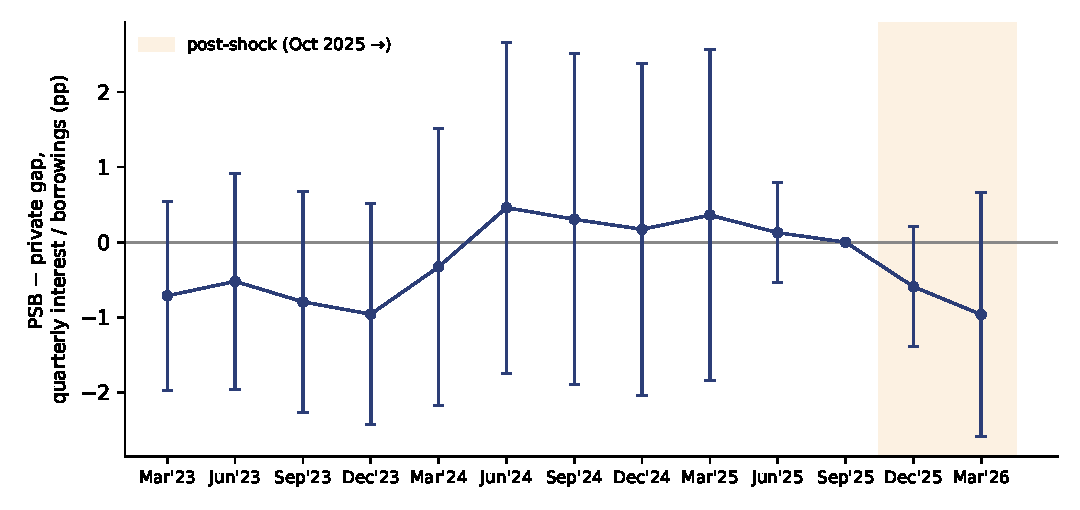
\includegraphics[width=0.92\textwidth]{tables/p_f1_eventstudy.pdf}
\caption{Pilot event study: the quarterly PSB$-$private gap in interest over borrowings,
relative to FY2026Q2 (the quarter before the sanctions). Whiskers are 95\% confidence
intervals (firm-clustered). Pre-shock coefficients hug zero; the gap turns negative in the
post-sanction quarters.}
\label{fig:p-es}
\end{figure}

\paragraph{Investment and targeting.} Table~\ref{tab:p-capex} reports capex (H2): the point
estimates are \emph{positive} throughout --- PSB-attached firms invest more post-shock, as
the shock-absorber view predicts. Under cluster-robust asymptotics the full-sample estimate
is insignificant ($t\approx1.5$), but under the exact randomization inference reported below
the share-weighted capex cushion has permutation $p=0.035$ --- a reminder that few-cluster
asymptotics can be noisy in either direction. We read H2 as \emph{supported by exact
inference but less settled than H1}: a consistently positive sign across all samples, exact
significance at 5\%, but magnitudes that move with sample composition. The triple-difference (Table~\ref{tab:p-ddd}) remains
uninformative because, within the sample, sector-level exposure has little variation to
exploit (most PSB and private firms sit in high-exposure sectors).

\paragraph{Inference with seventeen treated firms: randomization and placebo tests.}
Cluster-robust asymptotics are unreliable with few treated clusters, so we do not rest the
pilot's inference on them. Instead we report \textbf{exact Fisher randomization tests}:
holding the panel fixed, we reassign the treated label to a random set of seventeen of the
74 firms (or permute the continuous PSB share across firms), re-estimate the
difference-in-differences 2{,}000 times, and ask how often a placebo assignment produces a
coefficient as large as the observed one. Table~\ref{tab:p-inf}, Panel~A reports the exact
two-sided $p$-values: $0.062$ for the binary quarterly cost-of-debt cushion, $\mathbf{0.047}$
for the amount-weighted (share) version, and $\mathbf{0.035}$ for the share-weighted capex
cushion. Exact inference thus \emph{confirms} the cost-of-debt result at conventional levels
for the amount-weighted treatment --- the paper's preferred measure, since it uses the
facility values in the rating registry --- and reveals the capex cushion to be sharper than
its cluster-robust standard error suggested (asymptotic $t\approx1.5$, exact $p=0.035$),
consistent with few-cluster asymptotics being noisy in either direction. Panel~B implements
the placebo promised in Section~\ref{sec:strategy}: re-estimating the same specifications
with the shock moved one year earlier, on genuinely pre-shock data only. Every placebo
coefficient is wrong-signed (positive) and insignificant --- nothing happens at the false
date. One honest caveat: the permutation test assumes treatment assignment is exchangeable
across firms, whereas PSB-attached firms are somewhat more concentrated in high-exposure
sectors, so exchangeability holds only approximately; the quarter fixed effects and the
placebo-date test partially address this.

\begin{table}[t]
\centering
\begin{threeparttable}
\caption{Pilot inference: exact randomization tests and placebo shock dates}
\label{tab:p-inf}
\small
\begin{tabular}{lccc}
\toprule
\multicolumn{4}{l}{\emph{Panel A: randomization inference (exact permutation $p$, 2,000 draws)}} \\
 & Quarterly CoD & Quarterly CoD & Annual capex \\
 & (binary) & (share) & (share) \\
\midrule
Treatment $\times$ Post & -0.61 & -1.07 & 5.69 \\
Permutation $p$-value & [0.062] & [0.047] & [0.035] \\
\midrule
\multicolumn{4}{l}{\emph{Panel B: placebo shock one year earlier (pre-shock data only)}} \\
 & Quarterly CoD & Quarterly CoD & Annual CoD \\
 & (binary) & (share) & (binary) \\
\midrule
Treatment $\times$ Placebo post & 0.53 & 1.27 & 1.59 \\
 & (0.69) & (0.90) & (1.60) \\
\bottomrule
\end{tabular}
\begin{tablenotes}\footnotesize
\item Coefficients in percentage points, firm and time fixed effects throughout. Panel A:
exact two-sided permutation $p$-values in brackets, 2{,}000 draws, treated-set size (or the
empirical share distribution) held fixed. Panel B: placebo ``post'' = the two quarters (one
fiscal year) ending March 2025, estimated on pre-shock data only; firm-clustered SEs in
parentheses.
\end{tablenotes}
\end{threeparttable}
\end{table}

\paragraph{Who gets the cushion? A partial H4 test.} Public financials do permit one cut at
the allocation question that H4 poses, even without Prowess: we compute each firm's pre-shock
interest coverage (operating profit over interest) and split the cost-of-debt cushion by
whether the firm is below the sample median. The result points the same way as the Japanese
evidence: the cushion accrues to the \emph{financially stronger} PSB firms (PSB $\times$ Post
$=-3.2$ percentage points among stronger firms), and is \emph{offset} for weaker firms (the
PSB $\times$ Post $\times$ Weak interaction is $+5.8$ points, $t\approx2.3$), so weak PSB
firms receive essentially no cost-of-debt cushion. On its face this echoes the ``no zombie
tilt'' of \citet{lin2015government} --- the state cushion did not flow to the weakest
borrowers. We stress heavily that this rests on a seven-versus-ten-firm split, that
below-median coverage in a healthy large- and mid-cap sample is \emph{not} the zombie
(ICR $<1$) margin the hypothesis really targets, and that it is at best indicative. A genuine
zombie test --- the interpretive heart of the paper --- needs the firm-level exposure and the
thousands of firms, including the truly constrained ones, that only Prowess supplies.

\begin{table}[t]
\centering
\begin{threeparttable}
\caption{Pilot: state-bank attachment and capital expenditure}
\label{tab:p-capex}
\small
\begin{tabular}{lcc}
\toprule
Dep.\ var.: capex / lagged assets (\%) & (1) & (2) \\
\midrule
Treatment $\times$ Post & 3.24 & 5.69 \\
 & (2.45) & (3.70) \\
Treatment & Binary & Share \\
Firm FE, year FE & \checkmark & \checkmark \\
Observations & 287 & 287 \\
Firms & 74 & 74 \\
\bottomrule
\end{tabular}
\begin{tablenotes}\footnotesize
\item Firm and year fixed effects; SEs clustered by firm. Capex $=\Delta$(fixed
assets$+$CWIP)$+$depreciation, over lagged assets.
\end{tablenotes}
\end{threeparttable}
\end{table}

\begin{table}[t]
\centering
\begin{threeparttable}
\caption{Pilot: triple difference (sector-level exposure)}
\label{tab:p-ddd}
\small
\begin{tabular}{lcc}
\toprule
 & (1) CoD (\%) & (2) Capex (\%) \\
\midrule
PSB $\times$ Post & 0.65 & 12.90$^{***}$ \\
 & (1.04) & (1.41) \\
PSB $\times$ Post $\times$ HiExposure & 0.09 & -10.33$^{***}$ \\
 & (2.02) & (2.89) \\
Post $\times$ HiExposure & -1.00 & -0.11 \\
 & (1.23) & (1.68) \\
Firm FE, year FE & \checkmark & \checkmark \\
Observations & 287 & 287 \\
Firms & 74 & 74 \\
\bottomrule
\end{tabular}
\begin{tablenotes}\footnotesize
\item Firm and year fixed effects; SEs clustered by firm. Underpowered: exposure is
sector-level and near-constant within the disclosing sample.
\end{tablenotes}
\end{threeparttable}
\end{table}

\paragraph{What the pilot does and does not establish.}\label{sec:pilot-caveats}
The pilot delivers a genuine, public-data test of H1: the quarterly cost-of-debt cushion is
negative in every sample we built and significant at the 10\% level in the full seventeen-firm
sample (5\% in intermediate samples), with treatment amount-weighted from CRISIL
rating-rationale bank-lender annexures. H2 (investment) is suggestive --- positive throughout,
significant in intermediate samples, insignificant in the full sample. It remains indicative,
not decisive, and its limitations are real: (i) the treatment group is seventeen firms ---
the few-clusters inference problem this creates is addressed by the exact randomization
tests of Table~\ref{tab:p-inf}, but the effect remains sector-heterogeneous enough that
magnitudes move with sample composition (though never sign); (ii) firm coverage still depends on voluntary
disclosure or a CRISIL rating, a potential correlate of banking style; (iii) exposure is
sector- not firm-level; (iv) the cost-of-debt measure is an effective average rate, and
quarterly borrowings are held at the prior-year value; (v) the post-window is two quarters,
one partly reversed by the June accord; (vi) the longer quarterly pre-period is not perfectly
flat; and (vii) even mid-caps contain few ICR $<1$ firms, so H4 is untestable here. Every one
of these is resolved by the Prowess design of Section~\ref{sec:strategy}, which the skeletons
below pre-commit. The pilot establishes that the question is answerable on public Indian data,
that a state-bank cost-of-debt cushion is present and significant in this sample, and that the
full study is worth running --- not that the matter is settled.

\subsection{Pilot equity event study --- a falsification test}\label{sec:pilot-es}

The cost-of-debt pilot speaks to the \emph{creditor} margin. A cheap and independent
cross-check is available on the \emph{equity} margin, using free daily prices for the same
firms around the four precisely dated events of Section~\ref{sec:shock}: the sanctions
(22 Oct 2025), the Hormuz closure (28 Feb 2026), the naval blockade (13 Apr 2026), and ---
the falsification lever --- the Islamabad accord (17 Jun 2026) that \emph{resolved} the
shock. For each firm and event we compute a market-model cumulative abnormal return over
$[-1,+1]$ trading days (betas estimated on the prior 100 sessions against the NIFTY~50) and
regress it cross-sectionally on PSB attachment. If state-bank attachment were priced by
\emph{equity} holders as crisis insurance, its coefficient should be positive on the
adverse events and \emph{flip negative} on the relief day.

Table~\ref{tab:p-es} shows a nuanced picture that we report in full because the test was
pre-committed. The \emph{raw} PSB coefficient is a noisy near-zero at every event --- there
is no simple ``PSB firms did better'' effect in equity returns, and the relief-day sign-flip
does not appear. But the within-exposure interaction (PSB $\times$ HiExposure) is
\textbf{significantly positive at the sanctions announcement} ($+2.9$ percentage points,
$t\approx3.4$), the cleanest and least-anticipated of the four events: \emph{among}
energy-exposed firms, state-bank attachment cushioned the equity hit when the shock first
landed. The honest reading is that raw equity CARs conflate the banking relationship with
\emph{fundamentals} --- PSB-attached firms are more energy-exposed and cyclical, so a bare
PSB dummy mixes ``who they bank with'' and ``how exposed they are'' --- which is exactly why
the exposure-interacted coefficient, not the main effect, is where any cushion should and
does show up, and why the cost-of-debt DiD (with firm fixed effects) is the cleaner test.
The disciplined conclusion is unchanged: the state-bank cushion is clearest on the
\emph{cost of debt}; on equity it appears only for the most exposed firms and only at the
first shock, and we carry that limitation into the full study rather than paper over it.

\begin{table}[t]
\centering
\begin{threeparttable}
\caption{Pilot equity event study: PSB attachment and cumulative abnormal returns}
\label{tab:p-es}
\small
\begin{tabular}{lcccc}
\toprule
 & Sanctions & Hormuz & Blockade & Accord \\
 & (adverse) & (adverse) & (adverse) & (relief) \\
\midrule
PSB $\times$ event CAR (\%) & -0.98 & 0.78 & -0.07 & -0.79 \\
  & (0.64) & (1.39) & (1.18) & (0.75) \\
\midrule
PSB $\times$ HiExposure & 2.85$^{***}$ & -3.12$^{*}$ & -0.39 & 0.71 \\
  & (0.84) & (1.64) & (1.77) & (0.94) \\
\midrule
Firms & 73 & 73 & 73 & 73 \\
\bottomrule
\end{tabular}
\begin{tablenotes}\footnotesize
\item Market-model CARs over $[-1,+1]$ trading days, betas on the prior 100 sessions vs
NIFTY~50; free daily prices. Cross-sectional HC1-robust SEs in parentheses.
$^{*}/^{**}/^{***}$: 10/5/1\%. The raw PSB main effect is insignificant throughout; the
significant positive PSB $\times$ HiExposure at the sanctions indicates a cushion concentrated
among energy-exposed firms.
\end{tablenotes}
\end{threeparttable}
\end{table}

\subsection{Full study --- the cost of debt (H1)}\label{sec:full-cod}

Table~\ref{tab:cod} reports estimates of equation~\eqref{eq:did} for the cost of debt,
adding controls and tightening fixed effects across columns.

\begin{table}[t]
\centering
\begin{threeparttable}
\caption{State-bank attachment and the cost of debt around the 2025--26 shock}
\label{tab:cod}
\small
\begin{tabular}{lcccc}
\toprule
Dep.\ var.: Cost of debt (\%) & (1) & (2) & (3) & (4) \\
\midrule
PSB $\times$ Post                    & \tbd & \tbd & \tbd & \tbd \\
                                     & \tbd & \tbd & \tbd & \tbd \\
Controls                             &      & \checkmark & \checkmark & \checkmark \\
Firm FE                              & \checkmark & \checkmark & \checkmark & \checkmark \\
Quarter FE                           & \checkmark & \checkmark &  &  \\
Industry $\times$ quarter FE         &      &      & \checkmark & \checkmark \\
Sample                               & Full & Full & Full & Multi-bank \\
Observations                         & \tbd & \tbd & \tbd & \tbd \\
$R^2$                                & \tbd & \tbd & \tbd & \tbd \\
\bottomrule
\end{tabular}
\begin{tablenotes}\footnotesize
\item \TBDNOTE\ Standard errors clustered by firm in parentheses.
\end{tablenotes}
\end{threeparttable}
\end{table}

\subsection{Full study --- investment (H2)}

Table~\ref{tab:capex} repeats the design for the capex ratio; Figure~1 (event study,
equations~\eqref{eq:es}) plots the quarterly coefficients for both outcomes.

\begin{table}[t]
\centering
\begin{threeparttable}
\caption{State-bank attachment and capital expenditure around the 2025--26 shock}
\label{tab:capex}
\small
\begin{tabular}{lcccc}
\toprule
Dep.\ var.: Capex / lagged assets (\%) & (1) & (2) & (3) & (4) \\
\midrule
PSB $\times$ Post                    & \tbd & \tbd & \tbd & \tbd \\
                                     & \tbd & \tbd & \tbd & \tbd \\
Controls                             &      & \checkmark & \checkmark & \checkmark \\
Firm FE                              & \checkmark & \checkmark & \checkmark & \checkmark \\
Quarter FE                           & \checkmark & \checkmark &  &  \\
Industry $\times$ quarter FE         &      &      & \checkmark & \checkmark \\
Sample                               & Full & Full & Full & Multi-bank \\
Observations                         & \tbd & \tbd & \tbd & \tbd \\
$R^2$                                & \tbd & \tbd & \tbd & \tbd \\
\bottomrule
\end{tabular}
\begin{tablenotes}\footnotesize
\item \TBDNOTE\ Standard errors clustered by firm in parentheses.
\end{tablenotes}
\end{threeparttable}
\end{table}

\subsection{Full study --- targeting (H3)}

Table~\ref{tab:ddd} reports the triple difference~\eqref{eq:ddd} and constraint splits.

\begin{table}[t]
\centering
\begin{threeparttable}
\caption{Triple difference: exposure gradients and constraint heterogeneity}
\label{tab:ddd}
\small
\begin{tabular}{lcccc}
\toprule
& \multicolumn{2}{c}{Cost of debt} & \multicolumn{2}{c}{Capex ratio} \\
\cmidrule(lr){2-3}\cmidrule(lr){4-5}
& (1) & (2) & (3) & (4) \\
\midrule
PSB $\times$ Post                                  & \tbd & \tbd & \tbd & \tbd \\
PSB $\times$ Post $\times$ Exposure                & \tbd & \tbd & \tbd & \tbd \\
Post $\times$ Exposure                             & \tbd & \tbd & \tbd & \tbd \\
Constraint split                                   & None & High EFD & None & Small \\
Firm, industry $\times$ quarter FE, controls       & \checkmark & \checkmark & \checkmark & \checkmark \\
Observations                                       & \tbd & \tbd & \tbd & \tbd \\
\bottomrule
\end{tabular}
\begin{tablenotes}\footnotesize
\item \TBDNOTE\ EFD: external finance dependence \citep{rajan1998}.
\end{tablenotes}
\end{threeparttable}
\end{table}

\subsection{Full study --- allocation (H4)}

Table~\ref{tab:zombie} splits the sample by pre-shock interest coverage and reports the
sensitivity tests of Section~\ref{sec:strategy}.

\begin{table}[t]
\centering
\begin{threeparttable}
\caption{Who receives the cushion? Interest-coverage splits and efficiency tests}
\label{tab:zombie}
\small
\begin{tabular}{lcccc}
\toprule
& \multicolumn{2}{c}{Cost of debt} & Borrowing growth & Inv.--CF sens. \\
\cmidrule(lr){2-3}
& ICR $\geq 1$ & ICR $<1$ & ICR $<1$ share & $\Delta$ post \\
\midrule
PSB $\times$ Post              & \tbd & \tbd & \tbd & \tbd \\
                               & \tbd & \tbd & \tbd & \tbd \\
Observations                   & \tbd & \tbd & \tbd & \tbd \\
\bottomrule
\end{tabular}
\begin{tablenotes}\footnotesize
\item \TBDNOTE\ Column (3): share of post-shock PSB-client borrowing growth accruing to
pre-shock ICR $<1$ firms. Column (4): change in investment--cash-flow sensitivity
\citep{fazzari1988} for PSB-attached firms post-shock.
\end{tablenotes}
\end{threeparttable}
\end{table}

\subsection{Planned robustness}

Frozen alongside the main tables: (i) continuous PSB share and main-banker treatments;
(ii) entropy-balanced and matched samples on pre-shock observables; (iii) placebo shocks
at FY2024Q3 and FY2025Q3; (iv) exclusion of exporters (tariff channel) and of any firm
receiving scheme-specific support; (v) annual-frequency replication; (vi) two-way and
banker-level clustering; (vii) import-intensity as the alternative exposure margin.

%=====================================================================
\section{Conclusion}\label{sec:conclusion}

Japan's early-1990s crisis produced the sharpest evidence yet that government-owned banks
can function as shock absorbers rather than patronage machines
\citep{lin2015government}. India's 2025--26 energy shock --- externally imposed, precisely
dated twice over, unevenly felt in proportion to a pre-measurable firm characteristic, and
arriving in an economy with a genuine two-system split between state and private banking
relationships --- offers the natural second act, in the very economy where the normal-times value of
government-bank relationships is already established \citep{srinivasan2017}. This draft
has set out the institutional record, the data design, and a pre-specified identification
strategy whose central estimate, the triple-difference coefficient $\gamma$, is protected
against the confounders a contemporary policy environment supplies. The next version will
report the estimates. Whatever their sign, the allocation test carries the interpretation:
a cushion for viable constrained firms would extend the bright side of state banking to a
second country and a second century; a cushion for firms that cannot pay their interest
would show that the same aggregate insurance can be written on very different terms.

\newpage
\bibliography{references}

\newpage
\appendix
\section*{Data Appendix}
\addcontentsline{toc}{section}{Data Appendix}

\paragraph{Variable definitions.} Cost of debt: interest expense $/$ average total
borrowings, eq.~\eqref{eq:cod}. Capex ratio: cash-flow-statement purchases of fixed assets
$/$ lagged total assets. Energy exposure: power and fuel expense $/$ sales, FY2023--FY2025
average. Import intensity: imported raw materials $/$ total raw material expense, same
window. Leverage: total borrowings $/$ total assets. ICR: PBDIT $/$ interest expense.
All ratios winsorized at the 1st/99th percentiles.

\paragraph{PSB classification.} The twelve public sector banks (post April 2020):
State Bank of India; Bank of Baroda; Punjab National Bank; Canara Bank; Union Bank of
India; Indian Bank; Bank of India; Central Bank of India; Indian Overseas Bank; UCO Bank;
Bank of Maharashtra; Punjab \& Sind Bank. Banker strings are matched to these names and
their pre-merger constituents (e.g., Oriental Bank of Commerce and United Bank of India to
Punjab National Bank; Syndicate Bank to Canara Bank; Andhra Bank and Corporation Bank to
Union Bank; Allahabad Bank to Indian Bank; Dena Bank and Vijaya Bank to Bank of Baroda).
IDBI Bank, majority-owned by LIC and classified by the RBI as a private sector bank since
January 2019, is classified as private; robustness checks exclude IDBI-banked firms.
The full string-matching table ships with the replication package.

\paragraph{Shock chronology sources.} U.S.\ Treasury designation of Rosneft and Lukoil
(October 22, 2025); CREA monthly analyses of Russian fossil-fuel exports and sanctions
(January--May 2026) for import volumes and Urals pricing; contemporaneous market reporting
for VLCC rates, war-risk premia, Brent monthly averages, and the INR/USD path; Government
of India press releases for the ATF stabilization corpus and Export Promotion Mission;
Reserve Bank of India for the policy-rate path and banking aggregates. A dated source list
is maintained in the replication package.

\end{document}
